% Created by tikzDevice version 0.12 on 2019-04-13 14:06:18
% !TEX encoding = UTF-8 Unicode
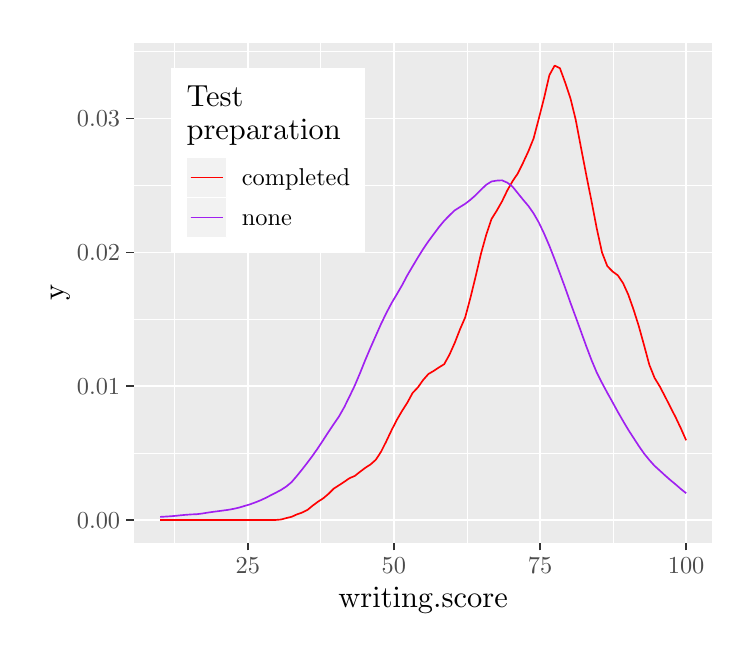
\begin{tikzpicture}[x=1pt,y=1pt]
\definecolor{fillColor}{RGB}{255,255,255}
\path[use as bounding box,fill=fillColor,fill opacity=0.00] (0,0) rectangle (252.94,216.81);
\begin{scope}
\path[clip] (  0.00,  0.00) rectangle (252.94,216.81);
\definecolor{drawColor}{RGB}{255,255,255}
\definecolor{fillColor}{RGB}{255,255,255}

\path[draw=drawColor,line width= 0.6pt,line join=round,line cap=round,fill=fillColor] (  0.00,  0.00) rectangle (252.94,216.81);
\end{scope}
\begin{scope}
\path[clip] ( 38.36, 30.72) rectangle (247.44,211.31);
\definecolor{fillColor}{gray}{0.92}

\path[fill=fillColor] ( 38.36, 30.72) rectangle (247.44,211.31);
\definecolor{drawColor}{RGB}{255,255,255}

\path[draw=drawColor,line width= 0.3pt,line join=round] ( 38.36, 63.10) --
	(247.44, 63.10);

\path[draw=drawColor,line width= 0.3pt,line join=round] ( 38.36,111.44) --
	(247.44,111.44);

\path[draw=drawColor,line width= 0.3pt,line join=round] ( 38.36,159.78) --
	(247.44,159.78);

\path[draw=drawColor,line width= 0.3pt,line join=round] ( 38.36,208.11) --
	(247.44,208.11);

\path[draw=drawColor,line width= 0.3pt,line join=round] ( 53.14, 30.72) --
	( 53.14,211.31);

\path[draw=drawColor,line width= 0.3pt,line join=round] (105.94, 30.72) --
	(105.94,211.31);

\path[draw=drawColor,line width= 0.3pt,line join=round] (158.74, 30.72) --
	(158.74,211.31);

\path[draw=drawColor,line width= 0.3pt,line join=round] (211.54, 30.72) --
	(211.54,211.31);

\path[draw=drawColor,line width= 0.6pt,line join=round] ( 38.36, 38.93) --
	(247.44, 38.93);

\path[draw=drawColor,line width= 0.6pt,line join=round] ( 38.36, 87.27) --
	(247.44, 87.27);

\path[draw=drawColor,line width= 0.6pt,line join=round] ( 38.36,135.61) --
	(247.44,135.61);

\path[draw=drawColor,line width= 0.6pt,line join=round] ( 38.36,183.95) --
	(247.44,183.95);

\path[draw=drawColor,line width= 0.6pt,line join=round] ( 79.54, 30.72) --
	( 79.54,211.31);

\path[draw=drawColor,line width= 0.6pt,line join=round] (132.34, 30.72) --
	(132.34,211.31);

\path[draw=drawColor,line width= 0.6pt,line join=round] (185.14, 30.72) --
	(185.14,211.31);

\path[draw=drawColor,line width= 0.6pt,line join=round] (237.94, 30.72) --
	(237.94,211.31);
\definecolor{drawColor}{RGB}{255,0,0}

\path[draw=drawColor,line width= 0.6pt,line join=round] ( 47.86, 38.93) --
	( 49.77, 38.93) --
	( 51.67, 38.93) --
	( 53.57, 38.93) --
	( 55.47, 38.93) --
	( 57.37, 38.93) --
	( 59.27, 38.93) --
	( 61.17, 38.93) --
	( 63.07, 38.93) --
	( 64.97, 38.93) --
	( 66.87, 38.93) --
	( 68.77, 38.93) --
	( 70.67, 38.93) --
	( 72.57, 38.93) --
	( 74.48, 38.93) --
	( 76.38, 38.93) --
	( 78.28, 38.93) --
	( 80.18, 38.93) --
	( 82.08, 38.93) --
	( 83.98, 38.93) --
	( 85.88, 38.93) --
	( 87.78, 38.93) --
	( 89.68, 38.93) --
	( 91.58, 39.09) --
	( 93.48, 39.61) --
	( 95.38, 40.07) --
	( 97.28, 40.93) --
	( 99.19, 41.60) --
	(101.09, 42.54) --
	(102.99, 44.10) --
	(104.89, 45.51) --
	(106.79, 46.73) --
	(108.69, 48.34) --
	(110.59, 50.24) --
	(112.49, 51.46) --
	(114.39, 52.71) --
	(116.29, 54.02) --
	(118.19, 54.82) --
	(120.09, 56.33) --
	(121.99, 57.76) --
	(123.90, 58.99) --
	(125.80, 60.68) --
	(127.70, 63.58) --
	(129.60, 67.37) --
	(131.50, 71.38) --
	(133.40, 75.10) --
	(135.30, 78.35) --
	(137.20, 81.32) --
	(139.10, 84.83) --
	(141.00, 86.82) --
	(142.90, 89.50) --
	(144.80, 91.66) --
	(146.70, 92.77) --
	(148.61, 94.04) --
	(150.51, 95.21) --
	(152.41, 98.64) --
	(154.31,102.89) --
	(156.21,107.78) --
	(158.11,112.16) --
	(160.01,119.30) --
	(161.91,127.06) --
	(163.81,135.17) --
	(165.71,142.01) --
	(167.61,147.67) --
	(169.51,150.70) --
	(171.41,154.05) --
	(173.32,158.01) --
	(175.22,161.35) --
	(177.12,164.15) --
	(179.02,168.02) --
	(180.92,172.11) --
	(182.82,176.81) --
	(184.72,184.04) --
	(186.62,191.46) --
	(188.52,199.67) --
	(190.42,203.10) --
	(192.32,202.18) --
	(194.22,196.98) --
	(196.12,191.34) --
	(198.03,183.53) --
	(199.93,173.53) --
	(201.83,163.69) --
	(203.73,154.20) --
	(205.63,144.29) --
	(207.53,135.60) --
	(209.43,130.68) --
	(211.33,128.72) --
	(213.23,127.33) --
	(215.13,124.53) --
	(217.03,120.32) --
	(218.93,114.95) --
	(220.83,108.95) --
	(222.74,102.03) --
	(224.64, 94.96) --
	(226.54, 90.24) --
	(228.44, 87.11) --
	(230.34, 83.47) --
	(232.24, 79.72) --
	(234.14, 76.01) --
	(236.04, 72.00) --
	(237.94, 67.71);
\definecolor{drawColor}{RGB}{160,32,240}

\path[draw=drawColor,line width= 0.6pt,line join=round] ( 47.86, 40.03) --
	( 49.77, 40.14) --
	( 51.67, 40.26) --
	( 53.57, 40.42) --
	( 55.47, 40.63) --
	( 57.37, 40.80) --
	( 59.27, 40.93) --
	( 61.17, 41.01) --
	( 63.07, 41.25) --
	( 64.97, 41.56) --
	( 66.87, 41.84) --
	( 68.77, 42.08) --
	( 70.67, 42.34) --
	( 72.57, 42.60) --
	( 74.48, 42.95) --
	( 76.38, 43.39) --
	( 78.28, 43.96) --
	( 80.18, 44.51) --
	( 82.08, 45.20) --
	( 83.98, 45.95) --
	( 85.88, 46.83) --
	( 87.78, 47.81) --
	( 89.68, 48.78) --
	( 91.58, 49.79) --
	( 93.48, 51.03) --
	( 95.38, 52.61) --
	( 97.28, 54.84) --
	( 99.19, 57.20) --
	(101.09, 59.64) --
	(102.99, 62.20) --
	(104.89, 64.90) --
	(106.79, 67.78) --
	(108.69, 70.73) --
	(110.59, 73.55) --
	(112.49, 76.31) --
	(114.39, 79.67) --
	(116.29, 83.53) --
	(118.19, 87.49) --
	(120.09, 91.97) --
	(121.99, 96.71) --
	(123.90,101.20) --
	(125.80,105.50) --
	(127.70,109.77) --
	(129.60,113.70) --
	(131.50,117.30) --
	(133.40,120.48) --
	(135.30,123.76) --
	(137.20,127.36) --
	(139.10,130.58) --
	(141.00,133.77) --
	(142.90,136.81) --
	(144.80,139.61) --
	(146.70,142.18) --
	(148.61,144.74) --
	(150.51,147.03) --
	(152.41,148.98) --
	(154.31,150.79) --
	(156.21,152.00) --
	(158.11,153.17) --
	(160.01,154.64) --
	(161.91,156.32) --
	(163.81,158.27) --
	(165.71,160.05) --
	(167.61,161.23) --
	(169.51,161.55) --
	(171.41,161.65) --
	(173.32,160.80) --
	(175.22,159.34) --
	(177.12,156.99) --
	(179.02,154.64) --
	(180.92,152.40) --
	(182.82,149.69) --
	(184.72,146.37) --
	(186.62,142.38) --
	(188.52,137.95) --
	(190.42,133.09) --
	(192.32,127.97) --
	(194.22,122.82) --
	(196.12,117.43) --
	(198.03,112.24) --
	(199.93,107.01) --
	(201.83,101.75) --
	(203.73, 96.73) --
	(205.63, 92.21) --
	(207.53, 88.44) --
	(209.43, 84.90) --
	(211.33, 81.49) --
	(213.23, 78.02) --
	(215.13, 74.71) --
	(217.03, 71.51) --
	(218.93, 68.57) --
	(220.83, 65.65) --
	(222.74, 62.91) --
	(224.64, 60.58) --
	(226.54, 58.45) --
	(228.44, 56.75) --
	(230.34, 54.99) --
	(232.24, 53.33) --
	(234.14, 51.76) --
	(236.04, 50.10) --
	(237.94, 48.58);
\end{scope}
\begin{scope}
\path[clip] (  0.00,  0.00) rectangle (252.94,216.81);
\definecolor{drawColor}{gray}{0.30}

\node[text=drawColor,anchor=base east,inner sep=0pt, outer sep=0pt, scale=  0.88] at ( 33.41, 35.90) {0.00};

\node[text=drawColor,anchor=base east,inner sep=0pt, outer sep=0pt, scale=  0.88] at ( 33.41, 84.24) {0.01};

\node[text=drawColor,anchor=base east,inner sep=0pt, outer sep=0pt, scale=  0.88] at ( 33.41,132.58) {0.02};

\node[text=drawColor,anchor=base east,inner sep=0pt, outer sep=0pt, scale=  0.88] at ( 33.41,180.92) {0.03};
\end{scope}
\begin{scope}
\path[clip] (  0.00,  0.00) rectangle (252.94,216.81);
\definecolor{drawColor}{gray}{0.20}

\path[draw=drawColor,line width= 0.6pt,line join=round] ( 35.61, 38.93) --
	( 38.36, 38.93);

\path[draw=drawColor,line width= 0.6pt,line join=round] ( 35.61, 87.27) --
	( 38.36, 87.27);

\path[draw=drawColor,line width= 0.6pt,line join=round] ( 35.61,135.61) --
	( 38.36,135.61);

\path[draw=drawColor,line width= 0.6pt,line join=round] ( 35.61,183.95) --
	( 38.36,183.95);
\end{scope}
\begin{scope}
\path[clip] (  0.00,  0.00) rectangle (252.94,216.81);
\definecolor{drawColor}{gray}{0.20}

\path[draw=drawColor,line width= 0.6pt,line join=round] ( 79.54, 27.97) --
	( 79.54, 30.72);

\path[draw=drawColor,line width= 0.6pt,line join=round] (132.34, 27.97) --
	(132.34, 30.72);

\path[draw=drawColor,line width= 0.6pt,line join=round] (185.14, 27.97) --
	(185.14, 30.72);

\path[draw=drawColor,line width= 0.6pt,line join=round] (237.94, 27.97) --
	(237.94, 30.72);
\end{scope}
\begin{scope}
\path[clip] (  0.00,  0.00) rectangle (252.94,216.81);
\definecolor{drawColor}{gray}{0.30}

\node[text=drawColor,anchor=base,inner sep=0pt, outer sep=0pt, scale=  0.88] at ( 79.54, 19.71) {25};

\node[text=drawColor,anchor=base,inner sep=0pt, outer sep=0pt, scale=  0.88] at (132.34, 19.71) {50};

\node[text=drawColor,anchor=base,inner sep=0pt, outer sep=0pt, scale=  0.88] at (185.14, 19.71) {75};

\node[text=drawColor,anchor=base,inner sep=0pt, outer sep=0pt, scale=  0.88] at (237.94, 19.71) {100};
\end{scope}
\begin{scope}
\path[clip] (  0.00,  0.00) rectangle (252.94,216.81);
\definecolor{drawColor}{RGB}{0,0,0}

\node[text=drawColor,anchor=base,inner sep=0pt, outer sep=0pt, scale=  1.10] at (142.90,  7.44) {writing.score};
\end{scope}
\begin{scope}
\path[clip] (  0.00,  0.00) rectangle (252.94,216.81);
\definecolor{drawColor}{RGB}{0,0,0}

\node[text=drawColor,rotate= 90.00,anchor=base,inner sep=0pt, outer sep=0pt, scale=  1.10] at ( 13.08,121.02) {y};
\end{scope}
\begin{scope}
\path[clip] (  0.00,  0.00) rectangle (252.94,216.81);
\definecolor{fillColor}{RGB}{255,255,255}

\path[fill=fillColor] ( 51.94,135.47) rectangle (121.99,202.28);
\end{scope}
\begin{scope}
\path[clip] (  0.00,  0.00) rectangle (252.94,216.81);
\definecolor{drawColor}{RGB}{0,0,0}

\node[text=drawColor,anchor=base west,inner sep=0pt, outer sep=0pt, scale=  1.10] at ( 57.44,188.23) {Test };

\node[text=drawColor,anchor=base west,inner sep=0pt, outer sep=0pt, scale=  1.10] at ( 57.44,176.35) { preparation};
\end{scope}
\begin{scope}
\path[clip] (  0.00,  0.00) rectangle (252.94,216.81);
\definecolor{drawColor}{RGB}{255,255,255}
\definecolor{fillColor}{gray}{0.95}

\path[draw=drawColor,line width= 0.6pt,line join=round,line cap=round,fill=fillColor] ( 57.44,155.43) rectangle ( 71.89,169.88);
\end{scope}
\begin{scope}
\path[clip] (  0.00,  0.00) rectangle (252.94,216.81);
\definecolor{drawColor}{RGB}{255,0,0}

\path[draw=drawColor,line width= 0.6pt,line join=round] ( 58.88,162.65) -- ( 70.45,162.65);
\end{scope}
\begin{scope}
\path[clip] (  0.00,  0.00) rectangle (252.94,216.81);
\definecolor{drawColor}{RGB}{255,0,0}

\path[draw=drawColor,line width= 0.6pt,line join=round] ( 58.88,162.65) -- ( 70.45,162.65);
\end{scope}
\begin{scope}
\path[clip] (  0.00,  0.00) rectangle (252.94,216.81);
\definecolor{drawColor}{RGB}{255,255,255}
\definecolor{fillColor}{gray}{0.95}

\path[draw=drawColor,line width= 0.6pt,line join=round,line cap=round,fill=fillColor] ( 57.44,140.97) rectangle ( 71.89,155.43);
\end{scope}
\begin{scope}
\path[clip] (  0.00,  0.00) rectangle (252.94,216.81);
\definecolor{drawColor}{RGB}{160,32,240}

\path[draw=drawColor,line width= 0.6pt,line join=round] ( 58.88,148.20) -- ( 70.45,148.20);
\end{scope}
\begin{scope}
\path[clip] (  0.00,  0.00) rectangle (252.94,216.81);
\definecolor{drawColor}{RGB}{160,32,240}

\path[draw=drawColor,line width= 0.6pt,line join=round] ( 58.88,148.20) -- ( 70.45,148.20);
\end{scope}
\begin{scope}
\path[clip] (  0.00,  0.00) rectangle (252.94,216.81);
\definecolor{drawColor}{RGB}{0,0,0}

\node[text=drawColor,anchor=base west,inner sep=0pt, outer sep=0pt, scale=  0.88] at ( 77.39,159.62) {completed};
\end{scope}
\begin{scope}
\path[clip] (  0.00,  0.00) rectangle (252.94,216.81);
\definecolor{drawColor}{RGB}{0,0,0}

\node[text=drawColor,anchor=base west,inner sep=0pt, outer sep=0pt, scale=  0.88] at ( 77.39,145.17) {none};
\end{scope}
\end{tikzpicture}
